% !TEX root = HW4.tex

\graphicspath{ {./images/} }

\newcommand{\spEighteenSvmOneA}{
	Below there is the plot showing the different examples in our dataset. 
	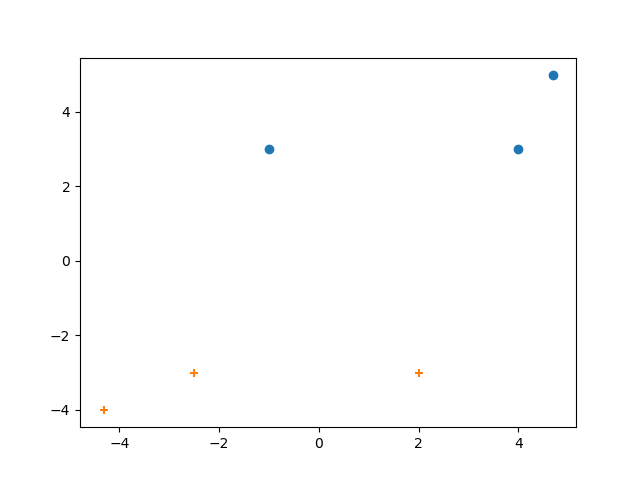
\includegraphics[scale=0.4]{hw4-plot.png}.
	
	Now it seems evident that the support vectors are (-1, 3), (4, 3), (-2.5, -3) and (2, -3). So the margin is defined by $x_2 = 3$ and $x_2 = -3$ and the width of the margin is 6. Since $\bw$ has to be perpendicular to the margin we have that $w_1 = 0$. Now to find $w_2$ we can use the relation
	\[ \frac{2}{||\bw||} = 6 \]
	Since $w_1 = 0$ we have that $w_2 = \frac{1}{3}$ and 
	\[ \bw = \begin{bmatrix}
		0\\
		\frac{1}{3}
	\end{bmatrix}\]
	To find $b$ we can use one of the support vectors, lets take (-1, 3):
	\[ (1)\left(0 \cdot -1 + \frac{1}{3} \cdot 3\right) + b = 1 \]
	Then $b = 0$.
}

\newcommand{\spEighteenSvmOneB}{
The support vectors are instances 1, 2, 3, 5.
}

\newcommand{\spEighteenSvmOneC}{
	Let $D$ be the number of dimensions of $\mathbf{x}$ and $N = |\cD|$ the number of elements in our data set.\\
	Lets first multiply the constraint by $-1$ so that we can match the components with the QP. \\
	\[ -y^{(i)}(\bw^\intercal\bx^{(i)} + b) \le -1 \]
	Since this is true for all $i$ we can write it in matrix form as follow
	\[
		-\begin{bmatrix}
			y^{(1)} & 0 & \cdots & 0\\
			\vdots  & \vdots  & \ddots & \vdots  \\
			0          & 0 & \cdots & y^{(N)}
		\end{bmatrix}
		\begin{bmatrix}
			x^{(1)} & 1\\
			\vdots & \vdots \\
			x^{(N)} & 1
		\end{bmatrix}
		\begin{bmatrix}
			\bw\\
			b
		\end{bmatrix} = 
		\begin{bmatrix}
			-1\\
			\vdots\\
			-1
		\end{bmatrix}
	\]
	where the first matrix is $N \times N$ and it is created by putting the $y^{(i)}$ in the $i$-th diagonal position; the second matrix is $N \times (D+1)$. \\
	Now we can take $\bz = \begin{bmatrix}
		\bw\\
		b
	\end{bmatrix}$.\\
	Then 
	\[
		G = -\begin{bmatrix}
			y^{(1)} & 0 & \cdots & 0\\
			\vdots  &    & \ddots & \vdots  \\
			0          & 0 & \cdots & y^{(N)}
		\end{bmatrix}
		\begin{bmatrix}
			x^{(1)} & 1\\
			\vdots & \vdots \\
			x^{(N)} & 1
		\end{bmatrix}
	\]
	\[
		\bf{h} = \begin{bmatrix}
			-1\\
			\vdots\\
			-1
		\end{bmatrix}
	\]
	Lets now remember that $||\bf{w}||^2$ can be written as $\bf{w}^\intercal \bf{w}$. 
	We can take $\bf{q}^\intercal = \begin{bmatrix}
		0 & \cdots & 0
	\end{bmatrix}$.
	
	Finally we want $\bz^\intercal P \bz$ to be $||\bw||^2$. 
	\begin{align*}
		\bz^\intercal P \bz &= 
			\begin{bmatrix}
				\bw & b
			\end{bmatrix}
			P
			\begin{bmatrix}
				\bw\\
				b
			\end{bmatrix}\\
		&= \begin{bmatrix}
				\bw & b
			\end{bmatrix}
			\begin{bmatrix}
				1 & 0 & \cdots & 0 & 0\\
				0 & 1 & \cdots & 0 & 0\\
				\vdots & \vdots & \ddots & 1 & 0\\
				0 & 0 & \cdots & 0 & 0
			\end{bmatrix}
			\begin{bmatrix}
				\bw\\
				b
			\end{bmatrix}
	\end{align*}
	So $P$ is a $(D+1)\times(D+1)$ matrix where the $D \times D$ upper-left matrix is an identity matrix and the last column and row are filled with zeros to get rid of the $b$.
}

\newcommand{\spEighteenSvmOneD}{
	When $C = \infty$ we are making the second term (the cost of the slack variables) to prevail over $\bf{w}$ so the minimization process will need to minimize the $\xi^{(i)}$. This means that it will try to find a separation that perfectly classifies all the data.\\
	
	When $C=0$ we are saying that we don't care about the slack variables at all. They can be anything so there may be many mis-classifications. Note that this is equivalent to hard-SVM because minimizing $||\bf{w}||$ is the same as maximizing the margin $\left(\frac{2}{||\bf{w}||}\right)$.
}

\newcommand{\spEighteenSvmOneE}{

}

\newcommand{\spEighteenSvmOneF}{

}

\newcommand{\spEighteenSvmTwoA}{
\newcommand{\xzPair}{\left( \bf{x}, \bf{z} \right)}
\begin{align*}
K_3\xzPair &= \alpha K_1\xzPair + \beta K_2\xzPair\\
&= \alpha \phi_1 \left( \bf{x} \right)^\intercal \phi_1\left(\bf{z} \right) + 
	\beta \phi_2 \left( \bf{x} \right)^\intercal \phi_2\left(\bf{z} \right)\\
&= \begin{bmatrix}
	\sqrt{\alpha}\phi_1 \left( \bf{x} \right)^\intercal\\
	\sqrt{\beta} \phi_2 \left( \bf{x} \right)^\intercal
\end{bmatrix} \begin{bmatrix}
	\sqrt{\alpha}\phi_1 \left( \bf{z} \right) &
	\sqrt{\beta} \phi_2 \left( \bf{z} \right)
\end{bmatrix}
\end{align*}
Therefore, we can define our new $\phi$ function in terms of $\phi_1$ and $\phi_2$. \\
Suppose $\phi_1(\cdot) \in \mathbb{R}^m$ and $\phi_2(\cdot) \in \mathbb{R}^n$
\[ \phi(\cdot) = \begin{bmatrix}
	\sqrt{\alpha}\phi_1 (\cdot) &
	\sqrt{\beta} \phi_2 (\cdot)
\end{bmatrix} \in \mathbb{R}^{m+n}\]
}

\newcommand{\spEighteenSvmTwoB}{
\begin{align*}
K \left(\bf{x}, \bf{z} \right) &= \left( \bf{x}^\intercal \bf{z} \right)^2\\
&= \left( x_1 z_1 + x_2 z_2  \right)^2\\
&= (x_1 z_1)^2 + 2x_1 x_2 z_1 z_2 + (x_2 z_2)^2\\
&= x_1^2 z_1^2 + 2x_1 x_2 z_1 z_2 + x_2^2 z_2^2\\
&= \begin{bmatrix}
 	x_1^2\\
	\sqrt{2}x_1 x_2\\
	x_2^2
\end{bmatrix}\begin{bmatrix}z_1^2 & \sqrt{2}z_1 z_2 & z_2^2\end{bmatrix}\\
&=\phi(\bf{x})^\intercal \phi(\bf{z})
\end{align*}
\[ \therefore \phi(\bf{a}) = \begin{bmatrix}a_1^2 & \sqrt{2}a_1 a_2 & a_2^2\end{bmatrix} \]
where \[ \bf{a} = \begin{bmatrix}a_1 &  a_2\end{bmatrix} \]
}